%% ****** Start of file apstemplate.tex ****** %
\documentclass[aps,prl,reprint,groupedaddress]{revtex4-2}

% You should use BibTeX and apsrev.bst for references
% Choosing a journal automatically selects the correct APS
% BibTeX style file (bst file), so only uncomment the line
% below if necessary.
% \bibliographystyle{apsrev4-2}

\usepackage{graphicx}
\usepackage{epstopdf}
\usepackage{amsmath}
\usepackage{amsthm}
\usepackage{amsfonts}
\usepackage{subfigure}
\usepackage{hhline}
\usepackage[left=1cm,right=1cm,top=1cm,bottom=1cm]{geometry}
\usepackage[miktex]{gnuplottex}
\usepackage{xcolor}
\usepackage{amssymb}
\usepackage{amsmath}
\usepackage{color}
\usepackage{hyperref}
\usepackage[percent]{overpic}
\usepackage{tikz}
\usepackage{tikz-3dplot}
\usepackage{mathrsfs}
\usepackage{wasysym}
\usepackage{tikz-cd}
\usepackage{caption}  % Elimina hypcap=true si está presente
\usepackage{stackengine,scalerel}
\usepackage{subcaption}


\usepackage{caption}
\captionsetup{skip=0pt}  % Reduce el espacio entre la imagen y su caption
\raggedbottom

% so sections, subsections, etc. become numerated.
\setcounter{secnumdepth}{3}

\newenvironment{Figura}
  {\par\medskip\noindent\minipage{\linewidth}}
  {\endminipage\par\medskip}

\renewcommand{\appendixname}{Apéndice} % Change "Appendix" to "Apéndice"

\begin{document}

%Title of paper
\title{
Trabajo Integrados - Autoencoder y Clasificador con PyTorch
}

% autores
\author{Kevin Gaston Mansilla}
\email[]{kevin.mansilla@mi.unc.edu.ar}

\affiliation{}

%fecha
\date{\today}

\begin{abstract}
En este trabajo se implementara un autoencoder convolucion que es una
herramienta muy útil para la reducción de dimensionalidad y la extracción de
características de las imágenes, ya que es capaz de capturar patrones generales
de las imágenes y comprimir la información de manera eficiente. Luego se
reutilizará el encoder del autoencoder previamente entrenado para entrenar un
clasificador convolucional desde cero y también solo entrenando los parámetros
de la capa clasificadora. Se realizaran experimentos variando los hiperparámetros
de la red para ver como afectan al error de reconstrucción y al desempeño del
clasificador para finalmente comparar los resultados obtenidos.
\end{abstract}

% insert suggested keywords - APS authors don't need to do this
%\keywords{}

%\maketitle must follow title, authors, abstract, and keywords
\maketitle

\section{Introducción}

Tomando como punto de partida la base de datos de Fashion MNIST
\footnote{https://github.com/zalandoresearch/fashion-mnist}, el objetivo de 
este trabajo es implementar un autoencoder convolucional que es basicamente 
un sistema de codificación y decodificación de imágenes. 

Luego de entrenar el autoencoder, procederemos a variar los hiperparámetros de 
la red para ver como afectan al error de reconstrucción. A su vez, definiremos y 
entrenaremos un clasificador convolucional reutilizando el encoder del 
autoencoder previamente entrenado. 

Por último, experimentaremos solo reentrenando los parametros de la capa 
clasificadora, dejando los parámetros de la capa codificadora tal como 
vienen entrenados del autoencoder convolucional y compararemos los resultados 
obtenidos.

\section{Autoencoder Convolucional}
En un autoencoder convolucional, se aplican convoluciones o filtros entre 
sucesivas capas de la red para reducir la dimensionalidad del problema. Estos 
filtros van a captar la información importante con la que realizaremos el encoder 
de la red para luego proceder a realizar el procedo inverso de la codificación,
es decir, la decodificación.

Como se muestra en la figura \ref{fig-autoencoder}, la principal funcion es 
entrenarlo para que reconstruya una imagen a partir de los datos normales con 
un error de reconstrucción menor posible. 

\begin{Figura}
  \centering
  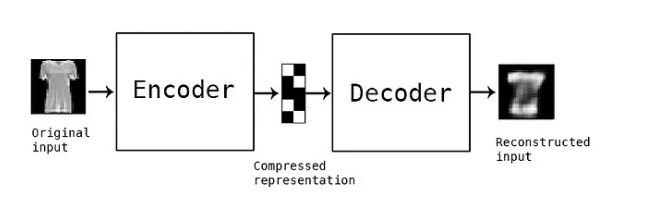
\includegraphics[width=1\textwidth]{figs/ejem_encoder_decoder.png}
  \captionof{figure}{Autoencoder convolucional}
  \label{fig-autoencoder}
\end{Figura}

Entrenaremos el autoencoder base con los siguientes hiperparámetros (modelo 
base):
\begin{itemize}
  \item [-] $n = 64$ (número de neuronas en la capa lineal).
  \item [-] $lr = 0.001$.
  \item [-] $p = 0.2$ (probabilidad de dropout).
  \item [-] $epochs = 15$.
  \item [-] $batch\_size = 100$.
  \item [-] $loss = MSELoss$.
  \item [-] $optimizer = Adam$.
\end{itemize}

La arquitectura del encoder es la siguiente:
\begin{itemize}
  \item Una capa convolucional 2D compuesta por:
  \begin{itemize}
    \item [-] un capa $Conv2d$ de entrada de dimensiones $(1, 28, 28)$ y de 
    salida $(16, 26, 26)$.
    \item [-] una capa de activación $ReLU$.
    \item [-] una capa $Dropout$.
    \item [-] una capa $MaxPool2d$, la cual mapea dimensiones $(16, 26, 26)$ a
    $(16, 13, 13)$.
  \end{itemize}
  \item Otra capa convolucional 2D compuesta por:
  \begin{itemize}
    \item [-] un capa $Conv2d$ de entrada de dimensiones $(16, 13, 13)$ y de 
    salida $(32, 11, 11)$
    \item [-] una capa de activación $ReLU$.
    \item [-] una capa $Dropout$.
    \item [-] una capa $MaxPool2d$, la cual mapea dimensiones $(32, 11, 11)$ a
    $(32, 5, 5)$.
  \end{itemize}
  \item Una capa lineal compuesta por:
  \begin{itemize}
    \item [-] una capa $Flatten$ que mapea dimensiones $(32, 5, 5)$ a $(800)$.
    \item [-] una capa $Linear$ de entrada $(800)$ y salida $n$.
    \item [-] una capa de activación $ReLU$.
    \item [-] una capa $Dropout$.
  \end{itemize}
\end{itemize}

El decoder con las siguientes capas:
\begin{itemize}
  \item Una capa lineal compuesta por:
  \begin{itemize}
    \item [-] una capa $Linear$ de entrada $n$ y salida $(800)$.
    \item [-] una capa de activación $ReLU$.
    \item [-] una capa $Dropout$.
    \item [-] una capa $Unflatten$ que mapea dimensiones $(800)$ a $(32, 5, 5)$.
  \end{itemize}
  \item Una capa convolucional 2D compuesta por:
  \begin{itemize}
    \item [-] un capa $ConvTranspose2d$ que mapea dimensiones $(32, 5, 5)$ a
    $(16, 13, 13)$.
    \item [-] una capa de activación $ReLU$.
    \item [-] una capa $Dropout$.
  \end{itemize}
  \item Otra capa convolucional 2D compuesta por:
  \begin{itemize}
    \item [-] un capa $ConvTranspose2d$ que mapea dimensione $(16, 13, 13)$ a
    $(1, 28, 28)$.
    \item [-] una capa de activación $Sigmoid$.
  \end{itemize}
\end{itemize}

No le agregamos capa de $Dropout$ en la capa de salida del decoder ya que 
este genera la salida reconstruida, que idealmente deberia ser lo más similar 
posible a los datos de entrada originales, si le agregaramos esta capa 
introduciria ruido que afectaria directamente la calidad de reconstrucción.

Luego variaremos los hiperparámetros de la red para ver como afecta su 
desempeño. Primero variamos la probabildidad de dropout a $0.1$, luego
cambiaremos el número de neuronas en la capa lineal a $256$ con el mismo 
dropout y finalmente cambiaremos el optimizador por SGD.

\section{Clasificador Convolucional}
Una vez entrenado el autoencoder, procederemos a reutilizar el encoder para
entrenar un clasificador convolucional. Que tendra la siguiente arquitectura:
\begin{itemize}
  \item Una capa lineal compuesta por:
  \begin{itemize}
    \item [-] una capa $Linear$ de entrada $n$ y salida $10$.
    \item [-] una capa de activación $ReLU$.
  \end{itemize}
\end{itemize}

El clasificador sera entrenado de dos formas. Primero reentrenaremos todos los
parámetros de la red y luego solo reentrenaremos los parámetros de la capa
clasificadora usando el encoder del autoencoder previamente entrenado.

\section{Resultados}
\subsection{Modelo sin entrenar}

En la figura \ref{fig-model-sin-entrenar} se muestra la imagen a predecir y las
imagenes reconstruidas por el modelo sin entrenar. Se puede observar que el
modelo no es capaz de reconstruir la imagen original.

\begin{Figura}
  \centering
  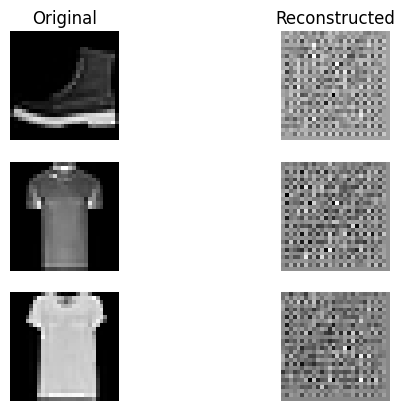
\includegraphics[width=0.5\textwidth]{figs1/modelo_sin_entrenar.png}
  \captionof{figure}{Imagenea a predir vs imagenes reconstruidas por el modelo 
  sin entrenar}
  \label{fig-model-sin-entrenar}
\end{Figura}

\subsection{Modelo base entrenado}

Los resultados obtenidos para el modelo base entrenado se presentan en la figura
\ref{fig-modelb-entrenado-perdida}. Se ve que las curvas muestran una 
disminución en la función de pérdida a medida que avanzan las épocas,pero a 
partir de la época $5$ las curvas comienzan a aumentar drasticamente, lo cual
podría ser un signo de que el modelo no va a tener un buen desempeño.
\begin{Figura}
  \centering
  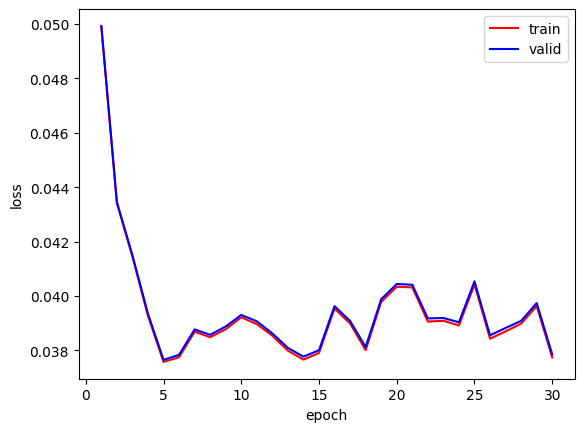
\includegraphics[width=0.60\textwidth]{figs1/modelo_original.png}
  \captionof{figure}{Función de pérdida del modelo base entrenado}
  \label{fig-modelb-entrenado-perdida}
\end{Figura}

En la figura \ref{fig-modelb-entrenado-img} se puede observar que el 
modelo es capaz de reconstruir la imagen original pero con una calidad no muy
buena, lo cual confirma lo observado en la función de pérdida.
\begin{Figura}
  \centering
  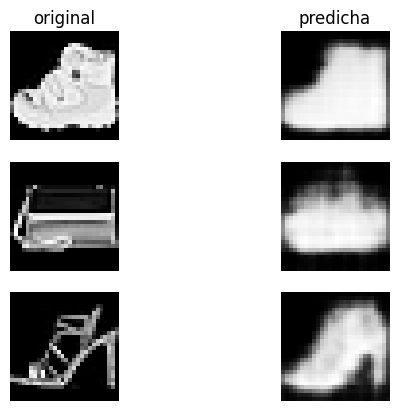
\includegraphics[width=0.5\textwidth]{figs1/test_modelo_original.png}
  \captionof{figure}{Imagenea a predir vs imagenes reconstruidas por el modelo
  base entrenado}
  \label{fig-modelb-entrenado-img}
\end{Figura}

\subsection{Modelo con probabilidad de dropout 0.1, $n=64$}

En la figura \ref{fig-model-dropout01} se muestra la función de pérdida del
modelo con probabilidad de dropout $0.1$. Podemos identificar un comportamiento 
similar al modelo base, por lo que el cambio de este hiperparámetro no afecta
significativamente el desempeño del modelo.
\begin{Figura}
  \centering
  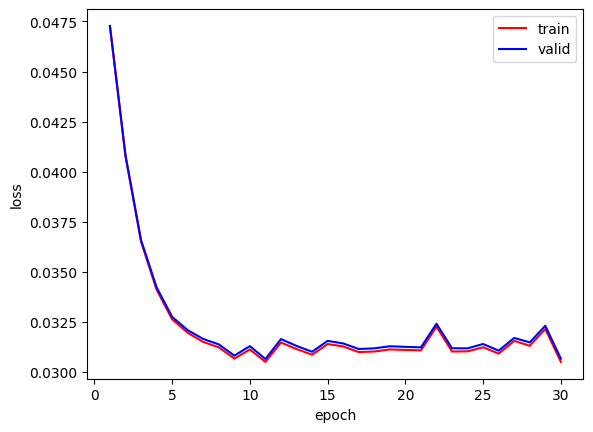
\includegraphics[width=0.60\textwidth]{figs1/modelo_n64_dropout01.png}
  \captionof{figure}{Función de pérdida del modelo con probabilidad de dropout 0.1}
  \label{fig-model-dropout01}
\end{Figura}

En la figura \ref{fig-model-dropout05b} vemos que el modelo es capaz de captar 
los patrones generales de las imágenes, pero pierde información de alto nivel, 
como los bordes o los detalles más finos.
\begin{Figura}
  \centering
  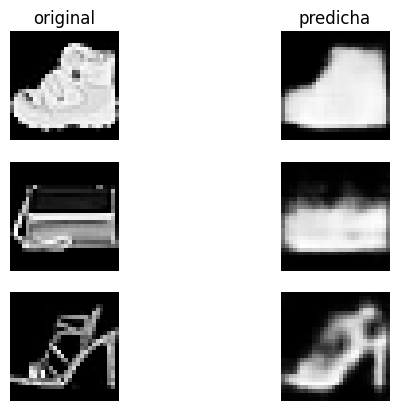
\includegraphics[width=0.5\textwidth]{figs1/test_modelo_n64_dropout_01.png}
  \captionof{figure}{Imagenea a predir vs imagenes reconstruidas por el modelo
  con probabilidad de dropout 0.1}
  \label{fig-model-dropout05b}
\end{Figura}

\subsection{Modelo con probabilidad de dropout 0.1, $n=256$}

Ahora con un dropout de $0.1$ y $n=256$ como vemos en la figura 
\ref{fig-model-dropout01} la funciones de perdida de ambos conjuntos de datos 
disminuyen constantemente, lo que indica el autoencoder está logrando comprimir 
y reconstruir los datos de entrada de manera eficiente. La proximidad entre las 
curvas muestra que el autoencoder esta funcionando correctamente, es decir, 
que las representaciones latentes que aprende son aplicables tanto al conjunto 
de entrenamiento como al de validación.
\begin{Figura}
  \centering
  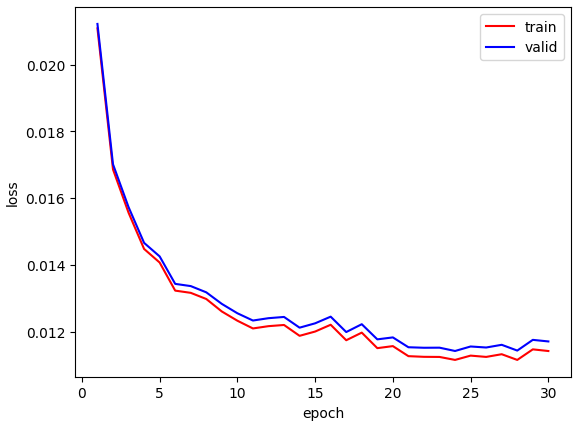
\includegraphics[width=0.60\textwidth]{figs1/modelo_n256_dropout01.png}
  \captionof{figure}{Función de pérdida del modelo con probabilidad de dropout 
  0.1 y $n=256$}
  \label{fig-model-dropout01-256}
\end{Figura}

En la figura \ref{fig-model-dropout05b} aunque no son perfectas, el modelo es 
capaz de capturar más detalles de las imágenes originales.
\begin{Figura}
  \centering
  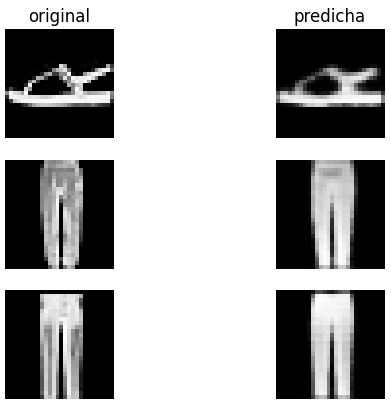
\includegraphics[width=0.5\textwidth]{figs1/test_modelo_n256_dropout01.png}
  \captionof{figure}{Imagenea a predir vs imagenes reconstruidas por el modelo
  con probabilidad de dropout 0.1 y $n=256$}
  \label{fig-model-dropout01b-256}
\end{Figura}

\subsection{Modelo con optimizador SGD}

Los resultados obtenidos para el modelo con optimizador SGD se presentan en la
figura \ref{fig-model-sgd} vemos que la función de pérdida del modelo 
disminuyen en ambos conjuntos de datos, lo cual podría indicar un buen 
comportamiento del modelo. Sin embargo, si observamos el eje de loss vemos que 
los valores son mucho mayores que en los modelos anteriores, lo cual indica que
el modelo no esta aprendiendo correctamente.
\begin{Figura}
  \centering
  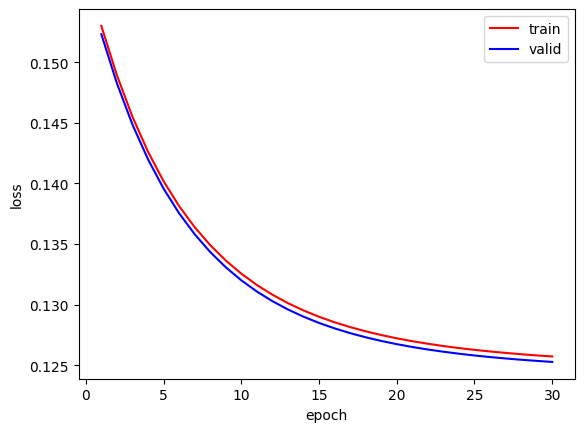
\includegraphics[width=0.60\textwidth]{figs1/modelo_con_sdg.png}
  \captionof{figure}{Función de pérdida del modelo con optimizador SGD}
  \label{fig-model-sgd}
\end{Figura}

En la figura \ref{fig-model-sgdb}. Se puede observar que el modelo no es capaz 
de reconstruir la imagen original.
\begin{Figura}
  \centering
  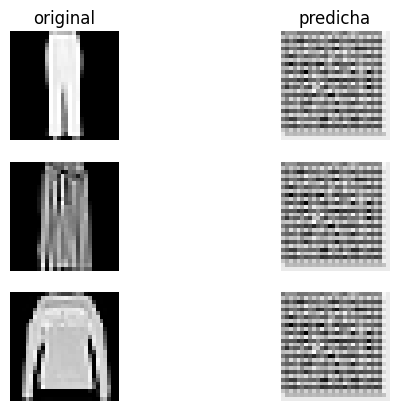
\includegraphics[width=0.5\textwidth]{figs1/test_modelo_sdg.png}
  \captionof{figure}{Imagenea a predir vs imagenes reconstruidas por el modelo SDG}
  \label{fig-model-sgdb}
\end{Figura}

\section{Clasificador Convolucional}

En esta sección se presentan los resultados obtenidos para el clasificador
convolucional que reutiliza el encoder del autoencoder previamente entrenado y 
en este caso se reentrenan todos los parámetros de la red por completo.

En la figura \ref{fig-clasificador-a} se muestran las funciones de perdidas 
tomando como partida el modelo base. Las curvas muestran una disminución en la 
función de pérdida tanto en el conjunto de entrenamiento como en el de validación 
a medida que avanzan las épocas con un error relativamente bajo, lo cual 
indica que le modelo mejora su capacidad de ajuste a los datos.
\begin{Figura}
  \centering
  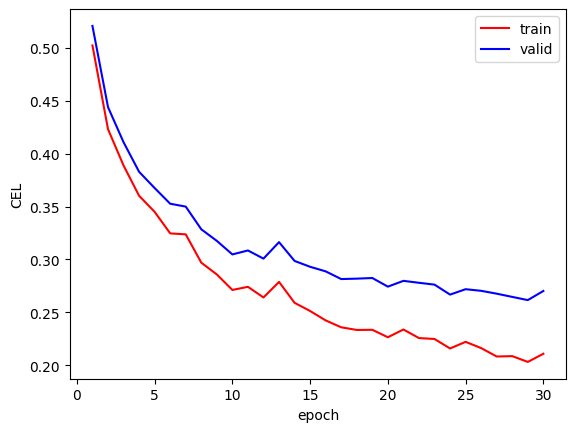
\includegraphics[width=0.60\textwidth]{figs1/modelo_con_clasificador_a.png}
  \captionof{figure}{Función de pérdida del clasificador}
  \label{fig-clasificador-a}
\end{Figura}

La precisión aumenta en ambos conjuntos de datos segun se muestra en la figura
\ref{fig-clasificador-b}, lo cual indica que el modelo es capaz de clasificar
correctamente las imágenes de entrada.
\begin{Figura}
  \centering
  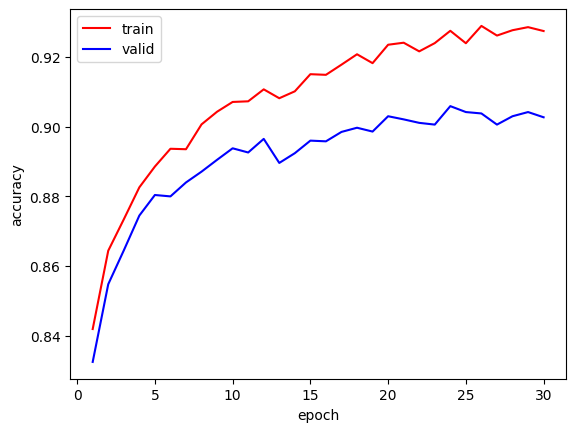
\includegraphics[width=0.60\textwidth]{figs1/modelo_con_clasificador_b.png}
  \captionof{figure}{Presición del clasificador}
  \label{fig-clasificador-b}
\end{Figura}

Y la matriz de confución se muestra en la figura \ref{fig-matrix}, donde se 
puede observar un buen desempeño del clasificador. En la diagonal principal se
encuentran los valores más altos, lo cual indica que la mayoría de las
predicciones son correctas. 

Se tiene un buen desempeño en clases como Trouser, Sandal, Sneaker, Bag y Ankle
Boot. Pero tiene dificultades en distingir entre las clases Shirt y Coat, 
ejemplo tomando la fila Shirt se ve que solo acierta 695 veces y 138 veces se 
equivoca prediciendo T-shirt y 83 como Pullover, algo similar ocurre con Coat, 
esto se debe a la similitud entre las categorías, ya que todas son prendas de 
vestir superiores.
\begin{Figura}
  \centering
  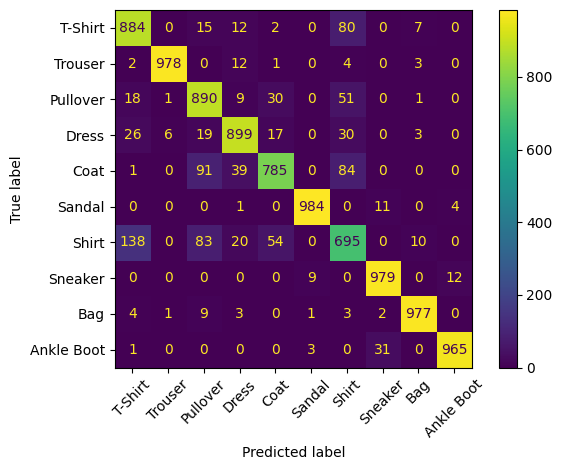
\includegraphics[width=0.75\textwidth]{figs1/matrix_confuncion_modelo_con_clasificador.png}
  \captionof{figure}{Matriz de confución del clasificador}
  \label{fig-matrix}
\end{Figura}

\subsection{Clasificador solo entrenando la capa clasificadora}

Ahora analizamos los resultados obtenidos para el clasificador convolucional
reutilizando el encoder del autoencoder previamente entrenado y en este caso
solo reentrenando los parámetros de la capa clasificadora. Es decir, que 
tomando como punto de partida el modelo base, solo se reentrenan los parámetros
de la capa clasificadora.

En la figura \ref{fig-clasificador-a-a} se muestran las funciones de perdidas 
de ambos conjuntos de datos y se observa que las curvas muestran una disminución
bastante pronunciada en ambos casos. El comportamiento es similar al modelo
anterior, pero con un error mucho mayor en la función de pérdida.
\begin{Figura}
  \centering
  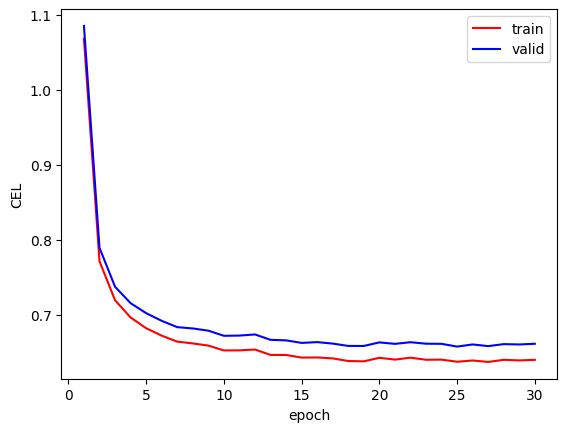
\includegraphics[width=0.60\textwidth]{figs1/modelo_original_entrenando_solo_clasificadora_a.png}
  \captionof{figure}{Función de pérdida del clasificador - solo reentrenando la capa clasificadora}
  \label{fig-clasificador-a-a}
\end{Figura}

En la figura \ref{fig-clasificador-a-b} se muestra la precisión del modelo en
ambos conjuntos de datos. Se observa un comportamiento diferente al modelo 
anterior. Inicialmente ambas curvas aumentan, pero luego se estabilizan y 
comienzan a oscilar.
\begin{Figura}
  \centering
  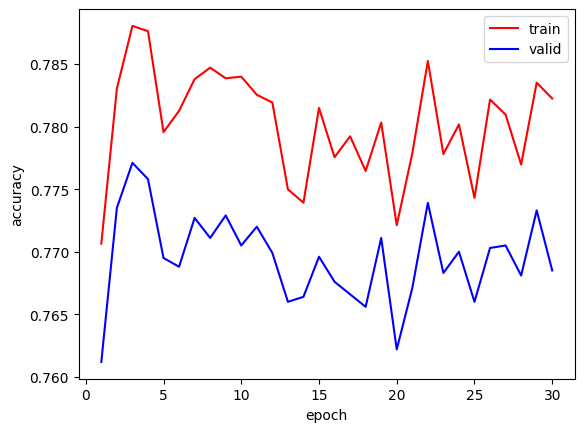
\includegraphics[width=0.60\textwidth]{figs1/modelo_original_entrenando_solo_clasificadora_b.png}
  \captionof{figure}{Presición del clasificador - solo reentrenando la capa clasificadora}
  \label{fig-clasificador-a-b}
\end{Figura}

A fin de comparar el desempeño de ambos clasificadores, se muestra en la figura
\ref{fig-matrix-a} la matriz de confución donde efectivamente se comprueba que 
el desempeño del clasificador solo reentrenando la capa clasificadora es peor
que el modelo anterior. Ya que los valores de la diagonal principal son menores
en todos las categorias. Y además empeora mucho el desempeño en las categorias 
Coat y Shirt.
\begin{Figura}
  \centering
  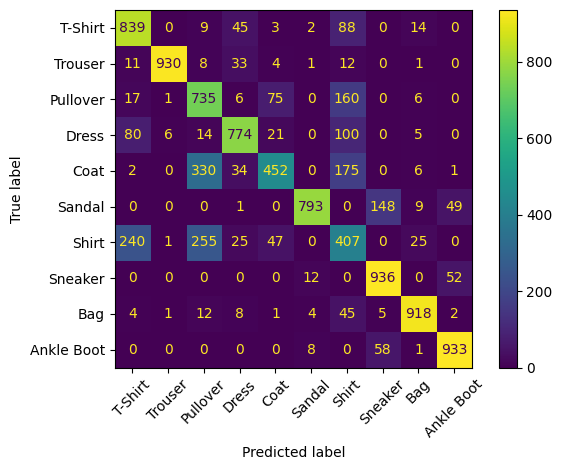
\includegraphics[width=0.75\textwidth]{figs1/matrix_confucion_modelo_original_entrenando_solo_clasificadora.png}
  \captionof{figure}{matrix de confución - solo reentrenando la capa clasificadora}
  \label{fig-matrix-a}
\end{Figura}

Entonces podemos concluir que el modelo base donde se reentrenan todos los
parámetros de la red tiene un mejor desempeño que el modelo donde solo se
reentrenan los parámetros de la capa clasificadora.

\section{Conclusiones}

A lo largo de este trabajo se fueron entrenando diferentes modelos de redes
neuronales convolucionales. Se comenzó con un autoencoder convolucional,
luego se reutilizó el encoder para entrenar un clasificador convolucional y
finalmente se compararon los resultados obtenidos al reentrenar solo la capa
clasificadora.

A medida que se fue aumentado la complejidad de los modelos los resultados
fueron mejorando, sin embargo se observó que las distancias entre las curvas
de entrenamiento y validación se fueron agrandando, lo cual indica signos de 
un desempeño no tan bueno.

El modelo base su desempeño al reconstruir las imágenes no fue muy bueno, aun 
que tenia un error relativamente bajo. Al variar la probabilidad de dropout a
$0.1$ no se observaron cambios significativos en el desempeño del modelo. Pero 
al aumentar el número de neuronas en la capa lineal a $256$ se observó una
mejora en la calidad de las imágenes reconstruidas.

El modelo con optimizador SGD no tuvo un buen desempeño, ya que el error de
reconstrucción fue muy alto. Por otro lado, el clasificador convolucional
reutilizando el encoder del autoencoder previamente entrenado tuvo un buen
desempeño, ya que al observar la matriz de confución se ve que la mayoría de las
predicciones son correctas. Por último, el clasificador solo reentrenando la
capa clasificadora tuvo un desempeño peor que el modelo anterior.

Algo muy importante a resaltar es que es muy dificil encontrar una combinación
de hiperparámetros que permita obtener un modelo con un desempeño óptimo, ya que
requiere de mucho tiempo y experiencia encontrar la combinación correcta.


\bibliography{ref}

% Specify following sections are appendices. Use \appendix* if there
% only one appendix.

%\onecolumngrid


\end{document}
%
% ****** End of file apstemplate.tex ******